% Script-aware BM25 for Urdu and Roman Urdu news search
% PLOS LaTeX template (plos_latex_template.tex, Version 3.8 Apr 2026)
%
% Official frozen system: M0. Do not headline SVM/MiniLM as the final retriever.
% Figures: PLOS submissions normally require separate figure files. The
% includegraphics calls compile a readable PDF; upload figures separately
% at submission (https://journals.plos.org/plosone/s/figures).

\documentclass[10pt,letterpaper]{article}
\usepackage[top=0.85in,left=1in,right=1in,footskip=0.75in]{geometry}
\usepackage{amsmath,amssymb}
\usepackage{changepage}
\usepackage{textcomp,marvosym}
\usepackage{cite}
\usepackage{nameref,hyperref}
\usepackage[right]{lineno}
\usepackage[nopatch=eqnum]{microtype}
\DisableLigatures[f]{encoding = *, family = * }
\usepackage[table]{xcolor}
\usepackage{array}
\usepackage{booktabs}
\usepackage{graphicx}
\usepackage{float}
\usepackage[aboveskip=1pt,labelfont=bf,labelsep=period,justification=raggedright,singlelinecheck=off]{caption}
\renewcommand{\figurename}{Fig}
\bibliographystyle{plos2025}

\makeatletter
\renewcommand{\@biblabel}[1]{\quad#1.}
\makeatother

\raggedright
\setlength{\parindent}{0.5cm}
\textwidth 5.25in
\textheight 8.75in

\usepackage{lastpage,fancyhdr}
\usepackage{epstopdf}
\pagestyle{fancy}
\fancyhf{}
\rfoot{\thepage/\pageref{LastPage}}
\renewcommand{\headrulewidth}{0pt}
\renewcommand{\footrule}{\hrule height 2pt \vspace{2mm}}
\fancyheadoffset[L]{2.25in}
\fancyfootoffset[L]{2.25in}
\lfoot{\today}

\begin{document}
\vspace*{0.2in}

\begin{flushleft}
{\Large
\textbf{Script-aware BM25 retrieval for Urdu and Roman Urdu news search}
}
\newline
\\
Hashim Shazad\textsuperscript{1*},
Adnan Aslam\textsuperscript{1}
\\
\bigskip
\textbf{1} Department of Creative Technologies, Air University, Islamabad, Pakistan
\\
\bigskip
* abbasihashim30@gmail.com
\end{flushleft}

\section*{Abstract}

Urdu news search is difficult because users type native Perso-Arabic script, informal Roman Urdu, or mixed forms, while many systems apply one retrieval path to every query. We freeze a script-aware lexical retriever, M0, over 111,860 news articles. A Unicode detector labels each query URDU, ROMAN, MIXED, or OTHER. URDU, MIXED, and OTHER queries search an Urdu BM25 index. ROMAN queries search a Method D romanized-document BM25 index. Queries are not rewritten. BM25 uses \(k_1=1.5\) and \(b=0.75\). Retrieval returns a Top-50 list; the official cutoff is Top-5.

On the development/validation known-item set, M0 achieved ExactSource Hit@5 of 87.18\% (68/78). On a newly sealed known-item set, it achieved 67.50\% (27/40). On a separate naturalistic query set evaluated by human relevance judgments, Success@5 was 57.50\% (23/40). These three percentages answer different questions and must not be averaged. Query-side expansions M1--M4 did not improve the 68/78 score; M0 remains the official frozen system. Roman Urdu is the main limitation (U Success@5: Urdu 17/18, Roman 6/18, mixed 0/4). We do not claim 87.18\% as unseen or human usefulness.

\clearpage
\newgeometry{top=0.85in,left=1in,right=1in,footskip=0.75in}
\linenumbers

\section*{Author summary}

People who search Urdu news often type either the native script or Roman Urdu (Urdu written with English letters). Those two forms do not match the same index. We freeze a simple, inspectable system: detect the script, search Urdu BM25 or a romanized BM25 index, and stop. We then measure three things separately. First, how often a known article is recovered on the freeze set (68/78). Second, how often that happens on new known-item queries (27/40). Third, how often a person finds something useful in the Top-5 of a natural query with no gold article (23/40). The first number is not the third. Roman queries remain much harder than Urdu-script queries.

\section*{Introduction}

Urdu is a major world language, yet it remains underserved in information retrieval (IR) research relative to English \cite{daud2017urdu,kazi2025urdu}. Users mix native Perso-Arabic script with Roman Urdu, whose spelling is unstandardized \cite{hussain2025qlora,mehmood2020xtreme,sitaram2019codeswitch}. A retriever that indexes only native-script text will miss Roman queries even when the article is in the collection.

The ULTRA framework of Bashir, Qaiser, and Hussain \cite{bashir2026ultra} provides a dual-embedding Urdu news architecture and a large news corpus. Its original switch is a static character-length threshold. Length does not decide which \emph{script index} to open. English work on query routing selects sparse versus dense retrieval \cite{arabzadeh2021predicting} or RAG depth \cite{jeong2024adaptiverag}; those systems were not designed for Roman Urdu.

This paper asks a narrower, measurable question. Freeze a lexical system. How often does it recover a known article on the development/validation pool? How often on a new sealed known-item sample? How often is the Top-5 useful when there is no gold article? Official retrieval here is BM25 with Unicode routing (M0). A companion historical study of SHORT/LONG SVM classification and MiniLM dual-index search is not the official retriever; we label it only where needed so that those numbers are not mistaken for M0.

\subsection*{Research questions}

\begin{itemize}
\item \textbf{RQ1.} Can a script-aware lexical pipeline (Urdu BM25 + Method D) recover known news articles from title-derived queries on a development/validation pool?
\item \textbf{RQ2.} Does that known-item score transfer to a newly sealed known-item sample written independently of the freeze set?
\item \textbf{RQ3.} How often is frozen M0 useful---at least one relevant or partially relevant document in the Top-5---on new naturalistic queries with no gold article?
\item \textbf{RQ4.} Do query-side Roman expansions M1--M4 improve development/validation ExactSource Hit@5 enough to replace M0?
\end{itemize}

\section*{Related work}

Daud et al.\ \cite{daud2017urdu} catalogue Urdu NLP obstacles: script, morphology, and limited standardized corpora. CURE \cite{iqbal2021cure} and a translated Urdu MS MARCO baseline \cite{butt2024urdumsmarco} supply evaluation resources; the latter reports MRR@10 of 0.247 under a different protocol than ours. Roman Urdu work is mostly classification \cite{hussain2025qlora,mehmood2020xtreme}. Multilingual dense retrieval can degrade off the pretraining head \cite{wu2024crosslingual,conneau2020xlmr}. BM25 remains a strong lexical baseline \cite{robertson2009bm25}. Query-adaptive routing in English selects among sparse, dense, or RAG strategies \cite{arabzadeh2021predicting,jeong2024adaptiverag,hsu2025dat} without a Roman Urdu path.

The gap we address is therefore not another English router. It is a frozen, hashed, script-conditional lexical retriever for Urdu news, evaluated with known-item ExactSource Hit@5 and naturalistic human Success@5 kept apart. We do not claim state of the art against CURE or Urdu MS MARCO.

\section*{Materials and methods}

\subsection*{Official frozen system (M0)}

Fig~\ref{fig:routing} summarizes M0. The corpus is \texttt{data/clean\_articles.csv} (\(n=111{,}860\)). The Roman dictionary is \texttt{models/roman\_urdu\_dict\_expanded.json} (198 keys). BM25 uses \(k_1=1.5\) and \(b=0.75\). Internally the system retrieves Top-50; the official cutoff is Top-5. Queries are not rewritten.

The detector counts Unicode Urdu letters (\texttt{U+0600}--\texttt{U+06FF}) and Latin letters. If both counts are zero the label is OTHER. If both are positive the label is MIXED. If only Urdu is positive the label is URDU. Otherwise the label is ROMAN. URDU, MIXED, and OTHER search Urdu BM25 over article text. ROMAN searches Method D BM25 over romanized documents (Phase 2 character table plus the reverse dictionary). The detector is not an SVM.

Corpus SHA-256: \texttt{8992a6acca3459eea17a7d7356dd490445daa00b958eab765713853c97a9f231}. Dictionary SHA-256: \texttt{30c3f61a64ec641abbb3acdbc7a8bcaf197f0238f1bf9e76c2c7ce8e590f86a3}.

\begin{figure}[H]
\centering
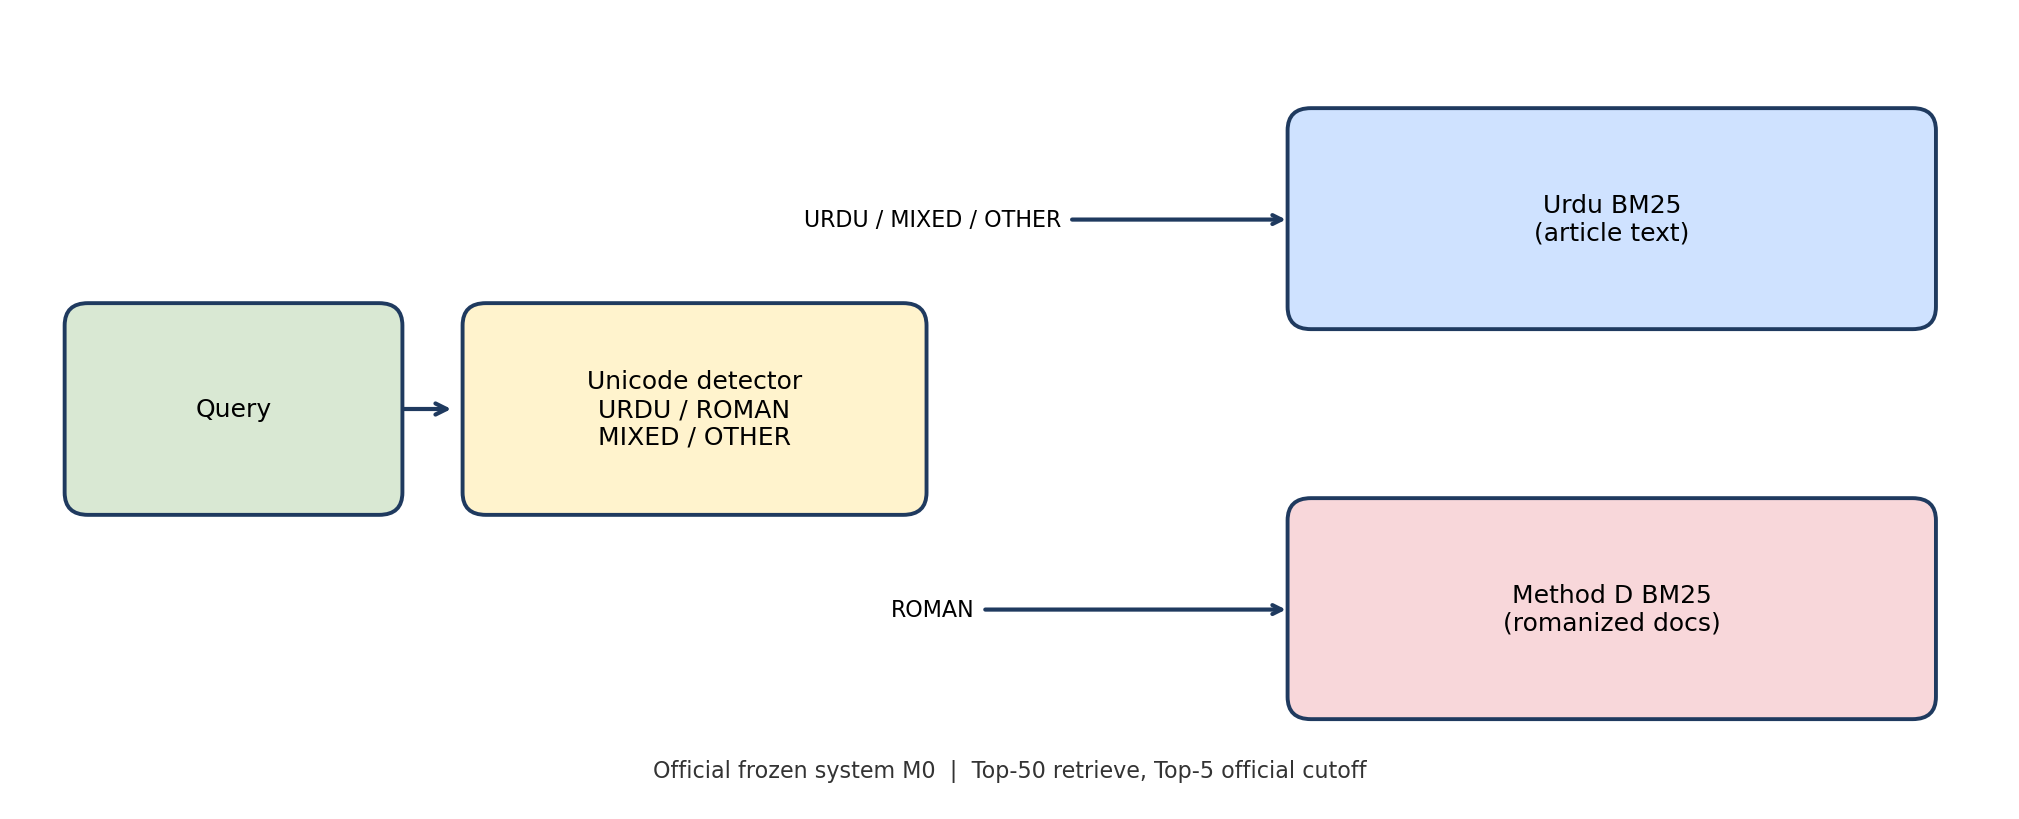
\includegraphics[width=0.95\linewidth]{figures/Fig1_m0_routing.png}
\caption{\textbf{Official frozen retriever M0.} Unicode script detection routes URDU, MIXED, and OTHER queries to Urdu BM25 and ROMAN queries to Method D romanized-document BM25. This is not an SVM SHORT/LONG router and not a MiniLM dual-index pipeline.}
\label{fig:routing}
\end{figure}

\subsection*{Evaluation metrics}

Known-item queries carry a pre-assigned source document id. ExactSource Hit@5 is 1 if and only if that source appears in the Top-5. Naturalistic queries have no source id. Human Success@5 is 1 if and only if at least one Top-5 document is labeled A (relevant) or B (partially relevant). These indicators are not interchangeable and are not averaged.

Secondary U metrics: conservative P@5 (count of A labels divided by 5), nDCG@5 with gains A\(=3\), B\(=2\), C\(=1\), D\(=\)E\(=0\), and MRR of the first A/B. nDCG@5 is not the usefulness headline: a topical C still has gain 1.

\subsection*{Development/validation known-item protocol}

Phase 2 \texttt{dev} + \texttt{internal\_val} (\(n=78\)) title-derived queries with source ids. Roman strings in this pool are \texttt{title\_roman}, not chat-style Roman Urdu. Method D was selected on that development Roman subset (22/23 ExactSource Hit@5 versus 0/23 for Method A). Urdu-only BM25 on the full pool (no Roman path) is 0.5897 ExactSource Hit@5. These comparators are development evidence for why a Roman index is required; they are not Phase 12 results.

\subsection*{Phase 11 ablation}

Query-side Roman expansions M1--M4 were scored on the same \(n=78\) pool. The freeze rule: replace M0 only if ExactSource Hit@5 improves. No test-set tuning on K or U.

\subsection*{Phase 12 sealed evaluation}

K001--K040 (new known-item) and U001--U040 (new naturalistic) were sealed before retrieval (seed 120260827). K uses ExactSource Hit@1/@5/@10/@50. U uses human Top-5 labels. No second retrieval after seeing labels. H001--H040 human Success@5 \(=25/40=62.5\%\) is a diagnostic on earlier trap queries; ExactSource Hit@5 is undefined on that set (no source id). It is not the official unseen usefulness result and must not be combined with U.

\subsection*{Historical Layer A (not official M0)}

Earlier work trained an SVM SHORT/LONG classifier and a MiniLM dual-index. Frozen Phase 3B classification was 86\% versus 84\% word-count; dual-index graded P@5 on H001--H040 did not improve over word count (SVM 33.00\% versus word count 36.50\%). Those figures are classification or dense-index pilots. They are not official M0 ExactSource Hit@5 or U Success@5. This manuscript does not present Layer A as the final ULTRA retriever.

\section*{Results}

Table~\ref{tab:official} reports the three official headlines. Do not average the rows.

\begin{table}[H]
\centering
\caption{\textbf{Official M0 results.} ExactSource Hit@5 and human Success@5 answer different questions. Do not average rows. Do not treat 87.18\% as unseen or human usefulness.}
\label{tab:official}
\begin{tabular}{p{4.2cm}p{3.4cm}p{3.2cm}l}
\toprule
\textbf{Evaluation} & \textbf{Dataset} & \textbf{Metric} & \textbf{Result} \\
\midrule
Development/validation known-item & Phase 2, \(n=78\) & ExactSource Hit@5 & 68/78 (87.18\%) \\
New known-item & K001--K040 & ExactSource Hit@5 & 27/40 (67.50\%) \\
New naturalistic (human) & U001--U040 & Success@5 & 23/40 (57.50\%) \\
\bottomrule
\end{tabular}
\end{table}

\subsection*{Development/validation known-item}

ExactSource Hit@5 \(=68/78=87.18\%\). This result is genuine for title-derived known-item search on that pool. It is not real-world accuracy, not human usefulness, and not unseen natural-query performance.

\subsection*{Phase 11}

M0, M1, M2, M3, and M4 all scored \(68/78=87.18\%\) ExactSource Hit@5. Roman-train Hit@5 remained \(61/64=95.31\%\). M1--M4 nDCG@5 was slightly below M0. M1 is a gate-passing candidate, not an improvement, and is not the official system.

\subsection*{New known-item (K001--K040)}

Table~\ref{tab:k} reports ExactSource Hit at multiple cutoffs. Primary metric: Hit@5 \(=27/40=67.50\%\). Descriptive detector split, not used for tuning: Urdu-script K titles 26/28; ordinary Roman titles 1/12. The drop from 87.18\% to 67.50\% is concentrated on ordinary Roman title queries, not on native-script Urdu BM25.

\begin{table}[H]
\centering
\caption{\textbf{Phase 12 K ExactSource results, frozen M0.} Primary metric is Hit@5. This evaluation does not replace 68/78 and is not human Success@5.}
\label{tab:k}
\begin{tabular}{lc}
\toprule
\textbf{Metric} & \textbf{Result} \\
\midrule
ExactSource Hit@1 & 20/40 (50.00\%) \\
ExactSource Hit@5 & 27/40 (67.50\%) \\
ExactSource Hit@10 & 28/40 (70.00\%) \\
ExactSource Hit@50 & 30/40 (75.00\%) \\
\bottomrule
\end{tabular}
\end{table}

\subsection*{Naturalistic human evaluation (U001--U040)}

Success@5 \(=23/40=57.50\%\). Conservative P@5 \(=0.2050\). nDCG@5 \(=0.6460\). MRR \(=0.4542\). This is human relevance, not ExactSource Hit@5. Conservative P@5 suggests many successes are a single useful document rather than a uniformly relevant Top-5.

Fig~\ref{fig:uscript} shows the descriptive script split: URDU 17/18, ROMAN 6/18, MIXED 0/4. Mixed \(n=4\) is too small for a population rate; it is reported because all four failed. These findings describe this sealed sample. They do not licence retuning Method D on U failures.

\begin{figure}[H]
\centering
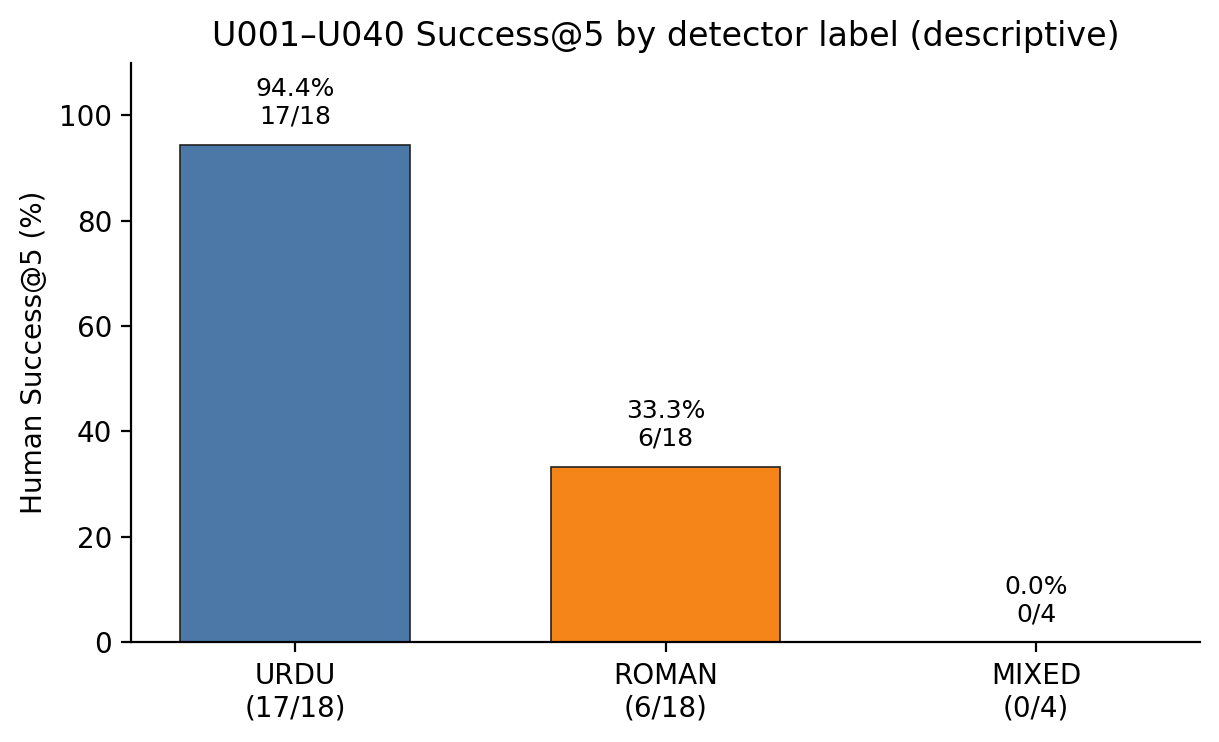
\includegraphics[width=0.85\linewidth]{figures/Fig2_u_script_split.png}
\caption{\textbf{Descriptive U Success@5 by detector label.} URDU 17/18, ROMAN 6/18, MIXED 0/4. Mixed \(n=4\) is descriptive only. This figure is not ExactSource Hit@5.}
\label{fig:uscript}
\end{figure}

\section*{Discussion}

87.18\% shows strong freeze-set known-item recovery, including development \texttt{title\_roman}. 67.50\% shows that score is not perfectly stable on independently sampled titles, especially ordinary Roman titles. 57.50\% asks a different question: on natural needs with no gold article, was anything in the Top-5 useful? Query mix matters: a Roman-heavy sample will look worse than an Urdu-only test even if the Urdu component is strong. Known-item evaluation alone cannot support a usefulness claim.

In official M0, adaptive routing is script-conditional index selection, not an SVM SHORT/LONG switch. Method D is necessary for title-roman-like known-item search on the development Roman subset and is insufficient for ordinary and chat Roman Urdu on new K and U. Phase 11 showed that small allowed query expansions did not move 68/78. Roman Urdu remains the major limitation of the frozen system.

\subsection*{Limitations}

K and U each have \(n=40\); point estimates have wide uncertainty. U labels are from one annotator; there is no inter-annotator agreement. The mixed-script subset is \(n=4\). The corpus is news only. M0 is lexical BM25 and does not rewrite queries. nDCG@5 with C-gain \(=1\) can look high when Success@5 fails. H001--H040 are diagnostic only. K, U, and H001--H040 are burned if M0 is changed. We do not claim 80\% unseen usefulness or 87.18\% real-world accuracy.

\subsection*{Conclusion}

M0 is a frozen script-aware BM25 news retriever. On the development/validation known-item set it achieved ExactSource Hit@5 of 87.18\% (68/78). On a newly sealed known-item set it achieved 67.50\% (27/40). On a separate naturalistic set, human Success@5 was 57.50\% (23/40). The contribution is that measured framework and its Roman Urdu limitation---not 87\% real-world accuracy.

\section*{Acknowledgments}

This manuscript reports MS thesis work at Air University, Islamabad, under Dr.\ Adnan Aslam. Funding, data, and author-contribution statements belong in the PLOS submission form.

\nolinenumbers
\bibliography{references}

\end{document}
